\documentclass[../main.tex]{subfile}
\graphicspath{{\subfix{../images}}}
\begin{document}

特征很重要。在过去的十年里,各种视觉识别任务的进展主要基于SIFT\cite{sift}和HOG\cite{hog}的使用。但是,如果我们看一下它们在典型的视觉识别任务的表现,即PASCAL VOC物体检测[15],人们普遍承认在2010-2012年期间进展缓慢,通过建立集合系统和采用成功方法的小变体获得了小的收益。

SIFT和HOG是顺时针方向的直方图,这种表示方法我们可以大致与V1的复杂细胞联系起来,V1是灵长类动物视觉通路的第一个皮质区域。但我们也知道,识别发生在下游的几个阶段,这表明可能有分层的、多阶段的过程来计算对视觉识别更有参考价值的特征。

Fukushima的 "neocognitron"[19],一个受生物启发的分层并具有移位不变性的模式识别模型,就是对这样一个过程的早期尝试。然而,neocognitron缺乏一个监督训练算法。在Rumelhart等人[33]的基础上,LeCun等人[26]表明,通过反向传播的随机梯度下降对训练卷积神经网络(CNN)是有效的,CNN是扩展neocognitron的一类模型。

CNN在20世纪90年代得到了大量使用(例如,\cite{classic_move}),但随后随着支持向量机的兴起而逐渐淡出人们的视野。2012年,Krizhevsky等人\cite{alexnet}在ImageNet大规模视觉识别挑战赛(ILSVRC)\cite{imagenet}上展示了大幅提高的图像分类准确性,重新点燃了人们对CNN的兴趣。他们的成功来自于在120万张标记图像上训练一个大型的CNN,以及对LeCun的CNN的一些改变(例如,ReLU非线性和dropout正则化)。

在ILSVRC 2012研讨会上,大家对ImageNet结果的意义进行了激烈的辩论。核心问题可以提炼为以下内容。ImageNet上的CNN分类结果在多大程度上可以推广到PASCAL VOC挑战赛的物体检测结果?

我们通过弥合图像分类和物体检测之间的差距来回答这个问题。本文首次表明,与基于更简单的类似HOG的特征的系统相比,CNN可以使PASCAL VOC的物体检测性能大幅提高。为了实现这一结果,我们重点研究了两个问题:用深度网络定位物体,以及用少量的注释检测数据训练一个大容量的模型。

与图像分类不同,检测需要对图像中的(可能是许多)物体进行定位。有一种方法将定位作为一个回归问题。然而,与我们同时进行的Szegedy等人[38]的工作表明,这种策略在实践中可能并不理想(他们报告说,2007年VOC的mAP为30.5\%,而我们的方法为58.5\%)。另一个选择是建立一个滑动窗口检测器。CNN已经以这种方式使用了至少20年,通常用于受限的物体类别,如人脸[32, 40]和行人[35]。为了保持高空间分辨率,这些CNN通常只有两个卷积层和池化层。我们也考虑过采用滑动窗口的方法。然而,在我们的网络中,有五个卷积层的高位单元在输入图像中具有非常大的感受野(195×195像素)和步长(32×32像素),这使得滑动窗口范式中的精确定位成为一个开放的技术挑战。

\begin{figure}[htb]
    \centering
    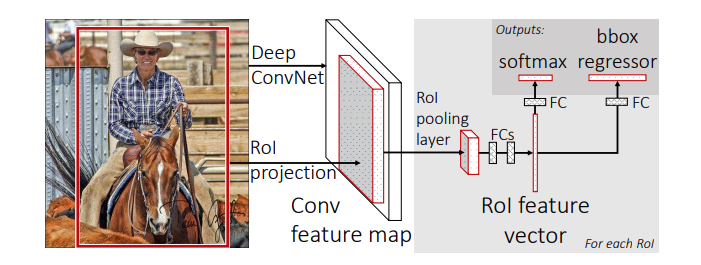
\includegraphics[width=\textwidth]{fig1.png}
    \caption{\textbf{物体检测系统概述。}我们的系统(1)接受一个输入图像,(2)提取大约2000个自下而上的区域候选,(3)使用一个大型卷积神经网络(CNN)计算每个候选的特征,然后(4)使用类别特定的线性SVM对每个区域进行分类。R-CNN在PASCAL VOC 2010上达到了53.7\%的平均精度(mAP)。作为比较,[39]报告说,使用相同的区域建议,但采用空间金字塔和视觉词汇袋的方法,达到了35.1\%的mAP。流行的可变形部分模型的表现为33.4\%。在200级ILSVRC2013检测数据集上,R-CNN的mAP为31.4\%,比OverFeat[34]有了很大的改进,它之前的最佳结果是24.3\%。}
    \label{fig:fig1}
\end{figure}

相反,我们通过“使用区域识别”范式[21]来解决CNN的定位问题,该范式在物体检测[39]和语义分割[5]中都很成功。在测试时,我们的方法为输入图像生成大约2000个与类别无关的候选区域,使用CNN从每个候选中提取一个固定长度的特征向量,然后用特定类别的线性SVM对每个区域进行分类。我们使用一种简单的技术(仿生图像扭曲)为每个候选区域计算得到一个固定大小的CNN输入,而不必考虑该区域的形状。图\ref{fig:fig1}展示了我们方法的概况,并强调了我们的一些结果。由于我们的系统将区域候选与CNN结合起来,我们将该方法称为R-CNN:具有CNN特征的区域。

在本文的更新版本中,我们通过在有200类的ILSVRC2013检测数据集上运行R-CNN,对R-CNN和最近提出的OverFeat\cite{overfeat}检测系统进行了正面的比较。OverFeat使用滑动窗口CNN进行检测,到目前为止是ILSVRC2013检测中表现最好的方法。我们表明,R-CNN明显优于OverFeat,其mAP为31.4\%而不是24.3\%。

检测中面临的第二个挑战是,标注的数据很少,目前可用的数据量不足以训练一个大型CNN。这个问题的传统解决方案是使用无监督的预训练,然后再进行有监督的微调(例如,[35])。本文的第二个主要贡献是表明,在一个大的辅助数据集(ILSVRC)上进行有监督的预训练,然后在一个小的数据集(PASCAL)上进行特定领域的微调,是在数据匮乏时学习大容量CNN的一个有效范式。在我们的实验中,检测的微调使mAP性能提高了8个百分点。经过微调,我们的系统在2010年的VOC上实现了54\%的mAP,而高度调整的、基于HOG的可变形部件模型(DPM)的mAP为33\%[17, 20]。我们还向读者指出Donahue等人[12]的同期工作,他们表明Krizhevsky的CNN可以作为一个黑盒特征提取器使用(不需要微调),在几个识别任务上产生出色的性能,包括场景分类、细粒度的子分类和领域适应。

我们的系统也是相当高效的。唯一针对类别的计算是一个相当小的矩阵-向量乘积和贪心非最大抑制。这一计算特性来自于所有类别共享的特征,这些特征也比以前使用的区域特征低两个数量级(参见[39])。

了解我们方法的失败模式对于改进它也很关键,因此我们报告了来自Hoiem等人[23]的检测分析工具的结果。作为这一分析的直接结果,我们证明了一个简单的边界盒回归方法大大减少了错误定位,而这是最主要的错误模式。

在发展技术细节之前,我们注意到,由于R-CNN是在区域上操作的,因此很自然地将其扩展到语义分割的任务中。经过细微的修改,我们在PASCAL VOC分割任务上也取得了有竞争力的结果,在VOC 2011测试集上的平均分割精度为47.9\%。

\end{document}